\documentclass[12pt, a4paper]{mycoursepaper}
\usepackage[a4paper,left=2.5cm,right=2cm,top=2cm,bottom=2cm,includefoot]{geometry}
\usepackage[utf8]{inputenc}
\usepackage[T1]{fontenc}
\usepackage[brazilian]{babel}
\usepackage{graphicx}
\usepackage{indentfirst}
\usepackage{array}
\usepackage{amsmath}
\usepackage{float}
\usepackage{multicol}
\usepackage{fancyhdr} 
\usepackage[usenames, dvipsnames]{color}
\usepackage[framed,numbered,autolinebreaks,useliterate]{mcode}
\usepackage{url,textcomp}
\usepackage[hidelinks]{hyperref}

\title{T03 Generate Random Data}
\author{Ricardo A. Fernandes}
\studentnumber{Matrícula: 2019105350 (PPGEC/CTEC/UFAL)}
\date{\today}
\college{Universidade Federal de Alagoas - UFAL\\
Instituto de Computação - IC\\
Programa de Pós-Graduação em  Informática - PPGI}
\coursename{Tópicos Especiais em Computação Visual e Inteligente: Aprendizagem Profunda}
\coursenumber{PPGI017-10}
\coursesection{-}
\instructor{Professor Tiago F. Vieira}

\newcommand{\norm}[1]{\lVert#1\rVert_2}

\begin{document}
\maketitle

\section{Gereção de Dados Randômicos}% \addtocounter{section}{1}
\vspace{-3mm}
Objetivo: Gerar dados randômicos de duas classes ``+'' e ``o'' usando numpy e matplotlib conforme ilustrado na Figura~\ref{fig:example}.
\vspace{-3mm}
\begin{itemize}
	\item use np.random.seed(1) para fixar a semente randômica e gerar distribuições mais próximas possíveis da Figura~\ref{fig:example}.
	\item Classe ``o'' tem média [0, 0].
	\item Classe ``+'' tem média [3, 4].
\end{itemize}
\vspace{-3mm}
\begin{figure}[H]
\centering
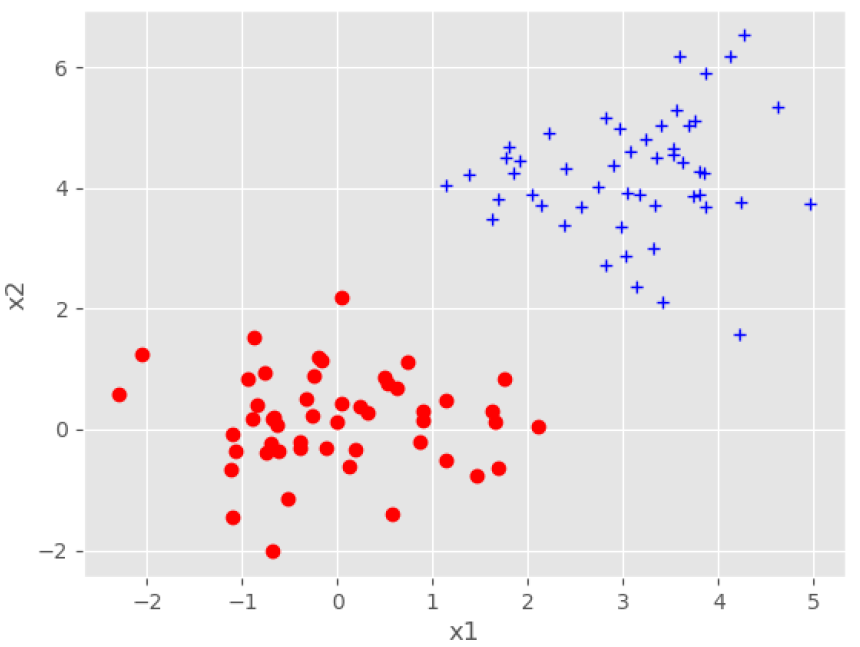
\includegraphics[width=0.45\paperwidth]{./example.png}
\caption{Ilustração das distribuições fornecidas para as classes ``o'' e ``+''.}
\label{fig:example}
\end{figure}

\newpage
\subsection{Resolução}
Desenvolveu-se a rotina generate\_random\_data.py (ver Listing~\ref{lst:grd}) em que se define a classe ``Data'' que recebe em seu construtor: nome, média e símbolo. A classe ``Data'' implementa também o método ``generate\_random\_sample'' que recebe um número de amostras e retorna dois arrays: $xs$ e $ys$. O método ``random.normal'' da numpy é utilizado para gerar os arrays $xs$ e $ys$, distribuições normais referentes às médias recebidas em cada direção, considerando desvio padrão unitário e o número de amostras fornecido.

Dessa forma, são criados os objetos $c$ e $p$, instâncias de ``Data'', representando as classes ``+'' e ``o'', respectivamente. Conforme orientação, utiliza-se a semente randômica 1 e chama-se o método ``generate\_random\_sample'' para ambos os objetos considerando 50 amostras. Os arrays retornados são plotados usando matplotlib, levando-se em consideração os nomes e símbolos previamente definidos.

% \lstinputlisting{../hellodl/generate_random_data.py}
\begin{lstlisting}[language=Python, caption=Rotina em Python3: generate\_random\_data.py, label=lst:grd]
import numpy as np
import matplotlib.pyplot as plt


class Data:  # define Data class
    def __init__(self, name, mean, mark):
        self.name = name,
        self.mean = mean
        self.mark = mark

    def generate_random_sample(self, n_samples):
        xs = np.random.normal(self.mean[0], 1, n_samples)
        ys = np.random.normal(self.mean[1], 1, n_samples)
        return xs, ys


c = Data('o', [0, 0], 'ro')  # circle instance
p = Data('+', [3, 4], 'b+')  # plus instance

# lock random seed
np.random.seed(1)

# generate samples
xc, yc = c.generate_random_sample(50)
xp, yp = p.generate_random_sample(50)

# plot samples
plt.plot(xc, yc, c.mark, label=c.name)
plt.plot(xp, yp, p.mark, label=p.name)

# set options and show plot
plt.xlabel('x1'), plt.ylabel('x2'), plt.grid(True)
plt.legend(loc='lower right')
plt.show()
\end{lstlisting}

\newpage
\subsection{Comparação entre as distribuições}

A Figura~\ref{fig:myrandomdata} ilustra as distribuições obtidas através da rotina generate\_random\_data.py utilizando o procedimento supracitado. Visualmente, observa-se boa concordância entre as distribuições geradas (ver Figura~\ref{fig:myrandomdata}) e as fornecidas (ver Figura~\ref{fig:example}).

\begin{figure}[H]
\centering
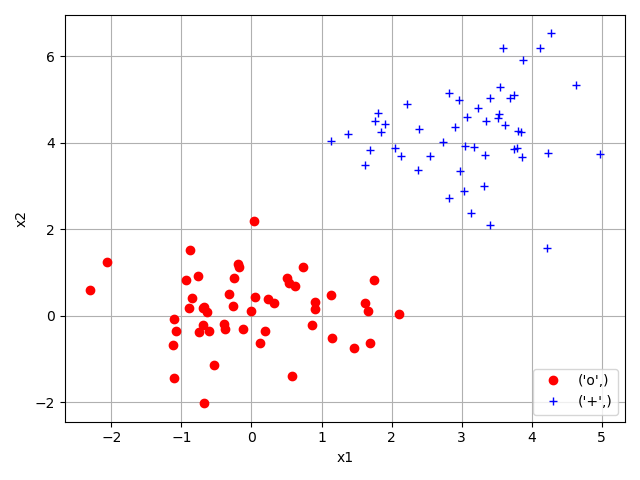
\includegraphics[width=0.45\paperwidth]{./myrandomdata.png}
\caption{Ilustração das distribuições geradas para as classes ``o'' e ``+''.}
\label{fig:myrandomdata}
\end{figure}

\begin{figure}[H]
\centering
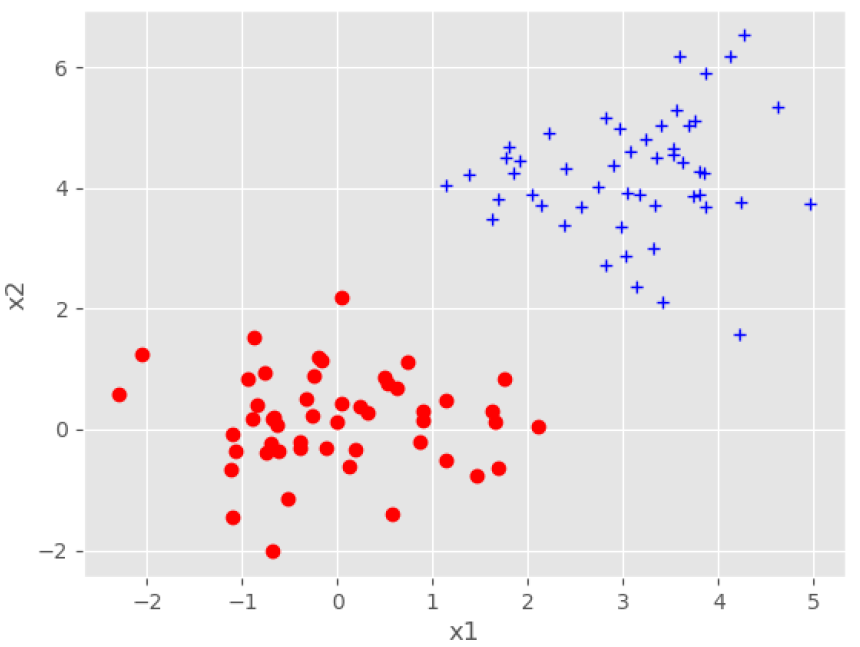
\includegraphics[width=0.45\paperwidth]{./example.png}
\caption{Ilustração das distribuições fornecidas para as classes ``o'' e ``+''.}
\label{fig:example}
\end{figure}

\end{document}
